\documentclass[dvipsnames]{article}%
\usepackage[T1]{fontenc}%
\usepackage[utf8]{inputenc}%
\usepackage{lmodern}%
\usepackage{textcomp}%
\usepackage{lastpage}%
\usepackage{geometry}%
\usepackage{graphicx}%
\usepackage{placeins}%
\usepackage{calc}%
\usepackage{tikz}%
\usepackage{xcolor}%
\usepackage{fancyhdr}%
\usepackage{booktabs}%
%
\usepackage[utf8]{inputenc}%
\usepackage[brazil]{babel}%
\setlength{\headsep}{3cm}%
\setlength{\footskip}{1cm}%
\geometry{top=4cm}%
\fancyhead[L]{
\includegraphics[width=0.1\paperwidth]{report_images/logo_2.png}}%
\fancyhead[R]{Relatóriio Termográfico}%
\fancyfoot[C]{GreTA®, Versão Beta - 2025 \quad Desenvolvido por Aisol}%
\usetikzlibrary{calc}%
%
\begin{document}%
\normalsize%
\thispagestyle{empty}%

\begin{tikzpicture}[overlay,remember picture]

% Rectangles
\shade[
left color=lightgray, 
right color=NavyBlue!40,
transform canvas ={rotate around ={45:($(current page.north west)+(0,-6)$)}}] 
($(current page.north west)+(0,-6)$) rectangle ++(9,1.5);

\shade[
left color=lightgray,
right color=lightgray!50,
rounded corners=0.75cm,
transform canvas ={rotate around ={45:($(current page.north west)+(.5,-10)$)}}]
($(current page.north west)+(0.5,-10)$) rectangle ++(15,1.5);

\shade[
left color=lightgray,
rounded corners=0.3cm,
transform canvas ={rotate around ={45:($(current page.north west)+(.5,-10)$)}}] ($(current page.north west)+(1.5,-9.55)$) rectangle ++(7,.6);

\shade[
left color=lightgray!80,
right color=blue!60,
rounded corners=0.4cm,
transform canvas ={rotate around ={45:($(current page.north)+(-1.5,-3)$)}}]
($(current page.north)+(-1.5,-3)$) rectangle ++(9,0.8);

\shade[
left color=RoyalBlue!80,
right color=blue!80,
rounded corners=0.9cm,
transform canvas ={rotate around ={45:($(current page.north)+(-3,-8)$)}}] ($(current page.north)+(-3,-8)$) rectangle ++(15,1.8);

\shade[
left color=lightgray,
right color=RoyalBlue,
rounded corners=0.9cm,
transform canvas ={rotate around ={45:($(current page.north west)+(4,-15.5)$)}}]
($(current page.north west)+(4,-15.5)$) rectangle ++(30,1.8);

\shade[
left color=RoyalBlue,
right color=Emerald,
rounded corners=0.75cm,
transform canvas ={rotate around ={45:($(current page.north west)+(13,-10)$)}}]
($(current page.north west)+(13,-10)$) rectangle ++(15,1.5);

\shade[
left color=lightgray,
rounded corners=0.3cm,
transform canvas ={rotate around ={45:($(current page.north west)+(18,-8)$)}}]
($(current page.north west)+(18,-8)$) rectangle ++(15,0.6);

\shade[
left color=lightgray,
rounded corners=0.4cm,
transform canvas ={rotate around ={45:($(current page.north west)+(19,-5.65)$)}}]
($(current page.north west)+(19,-5.65)$) rectangle ++(15,0.8);

\shade[
left color=RoyalBlue,
right color=red!80,
rounded corners=0.6cm,
transform canvas ={rotate around ={45:($(current page.north west)+(20,-9)$)}}] 
($(current page.north west)+(20,-9)$) rectangle ++(14,1.2);

% Year
\draw[ultra thick,gray]
($(current page.center)+(5,2)$) -- ++(0,-3cm) 
node[
midway,
left=0.25cm,
text width=5cm,
align=right,
black!75
]
{
{\fontsize{25}{30} \selectfont \bf Área \\[10pt] 1}
} 
node[
midway,
right=0.25cm,
text width=6cm,
align=left,
RoyalBlue]
{
{\fontsize{72}{86.4} \selectfont 2025}
};

% Title
\node[align=center] at ($(current page.center)+(0,-5)$) 
{
{\fontsize{60}{72} \selectfont {{Relatório Termográfico}}} \\[1cm]
{\fontsize{16}{19.2} \selectfont \textcolor{RoyalBlue}{ \bf Relatório Físico}}\\[3pt]};
\node[align=center] at ($(current page.center)+(0,-9.5)$) 
{ Desenvolvido por:};
\node[align=center] at ($(current page.center)+(0,-11)$) 
{
\includegraphics[width=0.4\paperwidth]{report_images/logo_2.png}};


\end{tikzpicture}%
\newpage%
\thispagestyle{empty}%
\vspace*{0.4cm}%
\rule{\linewidth}{0.5pt}%
\begin{center}%
{\large\bfseries Relatório de Inspeção por Imagem Térmica.  }%
\vspace*{0.5cm}%
\textbf{Responsável Técnico:} ANONIMIZADO, Engineer.  %
\textbf{CREA:} 12345678  %
\textbf{Date:} March 2025%
\textbf{Localização:} Campo Grande, MS. Brasil.  %
\textbf{Endereço:} Rua Manoel Inácio de Souza, n. 24, C.E.P : 79.020-220  %
\textbf{Software:} GreTA® - Georeferenced Thermographic Analysis System, Versão Beta.  %
\textbf{Versão:} Versão ANONIMIZADA  %
\end{center}%
\vspace*{0.4cm}%
\rule{\linewidth}{0.5pt}%
\vfill%
\noindent\textbf{Copyright © 2025 Aisol Soluções em Inteligência Artificial.  }%
Todos os direitos reservados. Nenhuma parte desta publicação pode ser reproduzida, distribuída ou transmitida sem autorização prévia.  %
\vspace*{0.2cm}%
\noindent\textbf{ISBN:} xxxxxxxx.  %
\textbf{Location:}%
Campo Grande, MS. Brasil.  %
Rua Manoel Inácio de Souza, n. 24.  %
C.E.P : 79.020{-}220.  %
\textbf{Copyrights:}%
Aisol, 2023.  %
\textbf{Release:}%
VERSAO ANONIMIZADA.  %
\textbf{Company:}%
Aisol Soluções em Inteligência Artificial em parceria com PVX Engenharia.  %
\newpage%
\tableofcontents%
\newpage%
\newpage%
\begin{abstract}%
As inspeções termográficas tornaram-se uma ferramenta essencial para avaliar o desempenho e a confiabilidade de usinas solares. Este estudo foca na detecção e análise de \textbf{pontos quentes (hotspots), diodos de bypass queimados e painéis ou strings inativos}, indicadores críticos de ineficiências operacionais. \textbf{Hotspots} aparecem como regiões de alta temperatura localizadas nos painéis solares, frequentemente causadas por sombreamento, acúmulo de sujeira ou células fotovoltaicas defeituosas, podendo levar à degradação do desempenho e danos a longo prazo. \textbf{Diodos de bypass queimados} interrompem o fluxo elétrico esperado, causando o superaquecimento de fileiras inteiras de células (\textbf{hot lines}), o que pode reduzir significativamente a eficiência do sistema. Além disso, \textbf{painéis ou strings inativos} — identificados como regiões mais frias do que o esperado nas imagens térmicas — indicam possíveis falhas em inversores, desconexões ou problemas elétricos. A detecção precoce e a implementação de ações corretivas direcionadas podem otimizar a geração de energia, prolongar a vida útil do sistema e prevenir falhas onerosas.%
\end{abstract}%
\pagestyle{fancy}%
\section{Introduction}%
A termografia, utilizando tecnologia infravermelha, é uma ferramenta fundamental para identificar discrepâncias térmicas em instalações solares. Este relatório emprega metodologias termográficas avançadas para detectar e localizar \textbackslash{}textbf\{pontos quentes (hotspots)\} em painéis solares e rastreadores. Esses hotspots, caracterizados por regiões de temperatura elevada, geralmente indicam anomalias operacionais ou ineficiências materiais na infraestrutura. \newline%
\newline%
A primeira seção do relatório, \textbackslash{}textbf\{Dados do Cliente\}, apresenta um conjunto de dados que inclui identificadores específicos do cliente e especificações dos equipamentos. Em seguida, a \textbackslash{}textbf\{Visão Geral da Área\} oferece uma representação espacial do local da instalação. Utilizando coordenadas geoespaciais, esta seção fornece um layout escalado dos painéis solares e rastreadores, estabelecendo uma matriz de referência. \newline%
\newline%
%
\section{Dados do Cliente}%
Anonimizado%
\section{Visão Geral da Área}%
 Nesta seção, apresentamos uma visão abrangente da área inspecionada. A \textbackslash{}textbf\{Figura 1\} exibe a \textbackslash{}textbf\{ortofoto\} montada a partir de todas as imagens capturadas da região. A \textbackslash{}textbf\{Figura 2\} apresenta uma representação esquemática da área, destacando as localizações dos rastreadores e dos hotspots detectados. A numeração dos rastreadores segue o padrão: da esquerda para a direita (de oeste para leste) e de cima para baixo (de norte para sul).%
\FloatBarrier%


\begin{figure}[h!]%
\centering%
\includegraphics[width=0.8\textwidth]{report_images/ortho.png}%
\caption{Ortofoto}%
\end{figure}

%
\FloatBarrier%


\begin{figure}[h!]%
\centering%
\includegraphics[width=0.8\textwidth]{report_images/layer_img.png}%
\caption{Máscara dos Painéis}%
\end{figure}

%
\FloatBarrier%


\begin{table}[h!]%
\caption{Resumo dos Defeitos Identificados}%
\begin{tabular}{lll}%
\toprule%
Tipo de Problema&Local do Painel&Coordenadas\\%
\midrule%
hotspots&13{-}20&{[}{-}40.56889903587372, {-}7.367918225916038{]}\\%
hotspots&13{-}10&{[}{-}40.568899328723454, {-}7.36779421175767{]}\\%
hotspots&10{-}53&{[}{-}40.569090925665385, {-}7.3683267901251375{]}\\%
hotspots&5{-}110&{[}{-}40.56940866763251, {-}7.3691199579623845{]}\\%
faultydiodes&6{-}68&{[}{-}40.569345265663955, {-}7.368599069454108{]}\\%
faultydiodes&6{-}26&{[}{-}40.569343215715776, {-}7.367989163757213{]}\\%
\bottomrule%
\end{tabular}%
\end{table}

%
\newpage%
\section{Pontos Quentes (Hot Spots)}%


\begin{figure}[h!]%
\begin{minipage}{0.31\linewidth}%
\centering%
\centering%
\includegraphics[width=\linewidth]{report_images/hotspots_13-20_map.jpg}%
\caption{Localização do defeito: 13-20}%
\end{minipage}%%
\hfill%
\begin{minipage}{0.31\linewidth}%
\centering%
\centering%
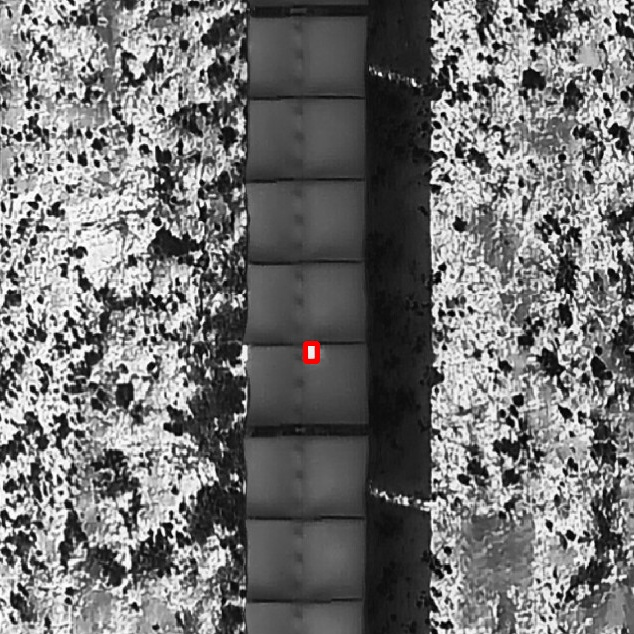
\includegraphics[width=\linewidth]{report_images/hotspots_13-20_cropped.jpg}%
\caption{Zoom no defeito: 13-20}%
\end{minipage}%%
\hfill%
\begin{minipage}{0.31\linewidth}%
\centering%
\centering%
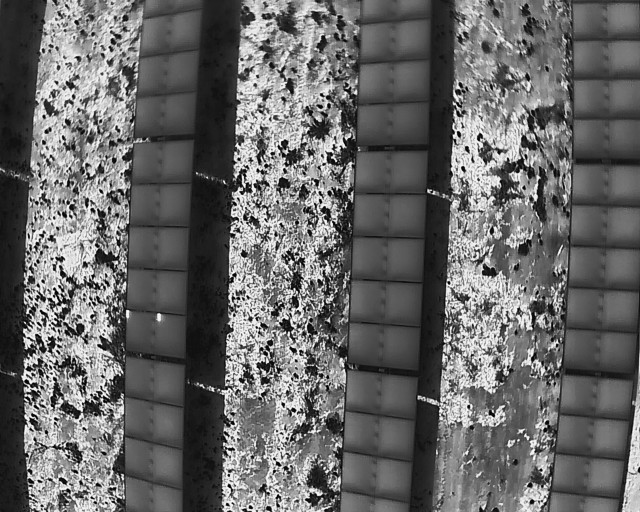
\includegraphics[width=\linewidth]{report_images/hotspots_13-20.jpg}%
\caption{Imagem Original: 13-20}%
\end{minipage}%
\end{figure}

%
\FloatBarrier%
No painel 13{-}20 há sinais de pontos quentes conforme as figuras acima.\newline%
%


\begin{figure}[h!]%
\begin{minipage}{0.31\linewidth}%
\centering%
\centering%
\includegraphics[width=\linewidth]{report_images/hotspots_13-10_map.jpg}%
\caption{Localização do defeito: 13-10}%
\end{minipage}%%
\hfill%
\begin{minipage}{0.31\linewidth}%
\centering%
\centering%
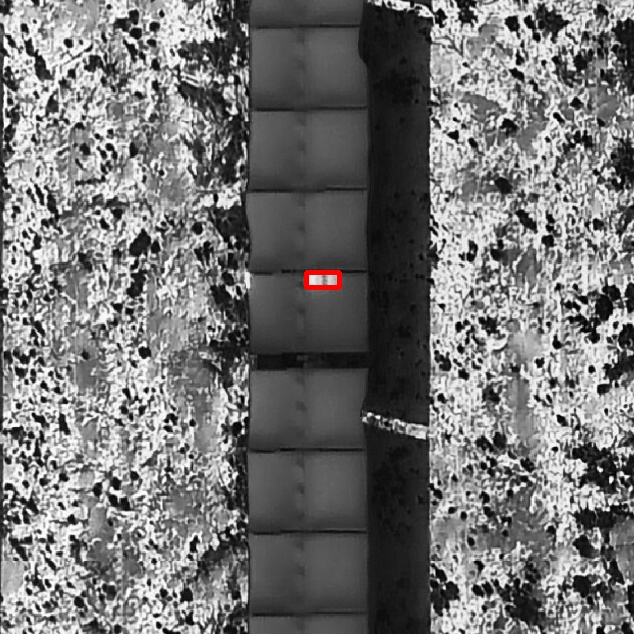
\includegraphics[width=\linewidth]{report_images/hotspots_13-10_cropped.jpg}%
\caption{Zoom no defeito: 13-10}%
\end{minipage}%%
\hfill%
\begin{minipage}{0.31\linewidth}%
\centering%
\centering%
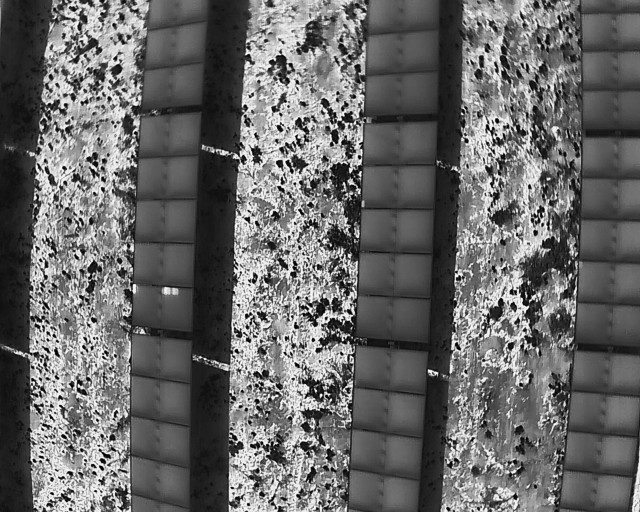
\includegraphics[width=\linewidth]{report_images/hotspots_13-10.jpg}%
\caption{Imagem Original: 13-10}%
\end{minipage}%
\end{figure}

%
\FloatBarrier%
No painel 13{-}10 há sinais de pontos quentes conforme as figuras acima.\newline%
%


\begin{figure}[h!]%
\begin{minipage}{0.31\linewidth}%
\centering%
\centering%
\includegraphics[width=\linewidth]{report_images/hotspots_10-53_map.jpg}%
\caption{Localização do defeito: 10-53}%
\end{minipage}%%
\hfill%
\begin{minipage}{0.31\linewidth}%
\centering%
\centering%
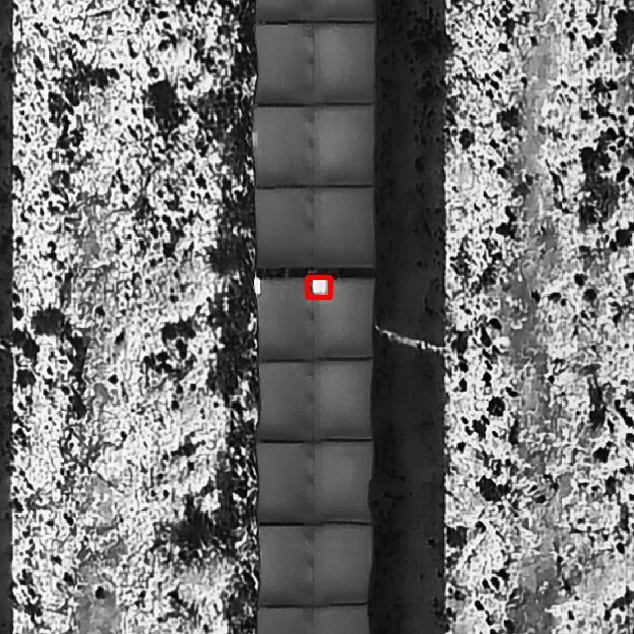
\includegraphics[width=\linewidth]{report_images/hotspots_10-53_cropped.jpg}%
\caption{Zoom no defeito: 10-53}%
\end{minipage}%%
\hfill%
\begin{minipage}{0.31\linewidth}%
\centering%
\centering%
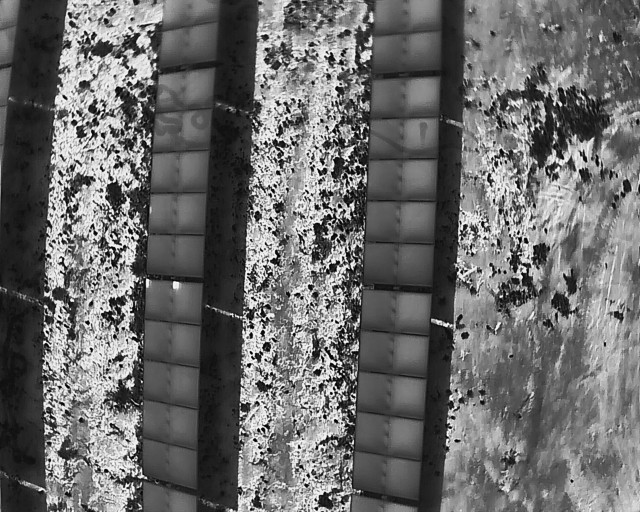
\includegraphics[width=\linewidth]{report_images/hotspots_10-53.jpg}%
\caption{Imagem Original: 10-53}%
\end{minipage}%
\end{figure}

%
\FloatBarrier%
No painel 10{-}53 há sinais de pontos quentes conforme as figuras acima.\newline%
%


\begin{figure}[h!]%
\begin{minipage}{0.31\linewidth}%
\centering%
\centering%
\includegraphics[width=\linewidth]{report_images/hotspots_5-110_map.jpg}%
\caption{Localização do defeito: 5-110}%
\end{minipage}%%
\hfill%
\begin{minipage}{0.31\linewidth}%
\centering%
\centering%
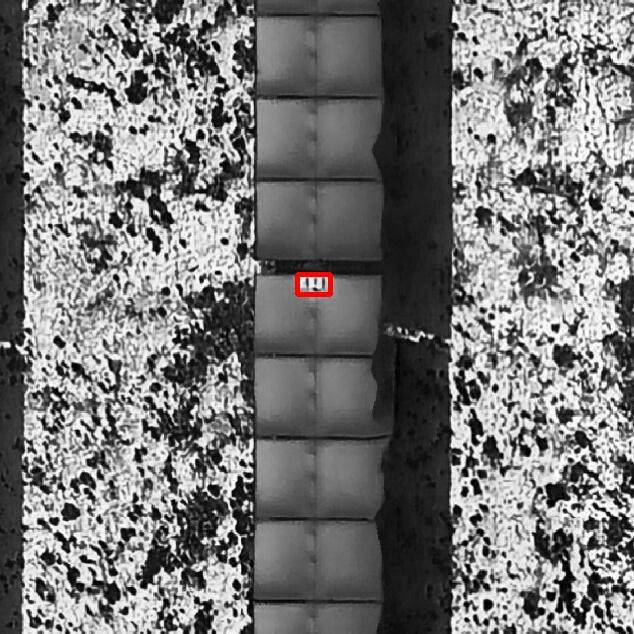
\includegraphics[width=\linewidth]{report_images/hotspots_5-110_cropped.jpg}%
\caption{Zoom no defeito: 5-110}%
\end{minipage}%%
\hfill%
\begin{minipage}{0.31\linewidth}%
\centering%
\centering%
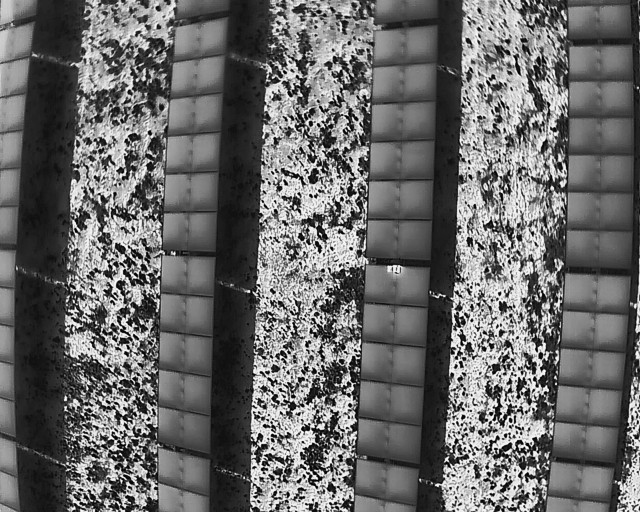
\includegraphics[width=\linewidth]{report_images/hotspots_5-110.jpg}%
\caption{Imagem Original: 5-110}%
\end{minipage}%
\end{figure}

%
\FloatBarrier%
No painel 5{-}110 há sinais de pontos quentes conforme as figuras acima.\newline%
%
\newpage%
\section{Painéis Desligados}%
As imagens coletadas não detectaram painéis desligados na área inspecionada.\newline%
%
\newpage%
\section{Diodos de Bypass Queimados}%


\begin{figure}[h!]%
\begin{minipage}{0.31\linewidth}%
\centering%
\centering%
\includegraphics[width=\linewidth]{report_images/faultydiodes_6-68_map.jpg}%
\caption{Localização do defeito: 6-68}%
\end{minipage}%%
\hfill%
\begin{minipage}{0.31\linewidth}%
\centering%
\centering%
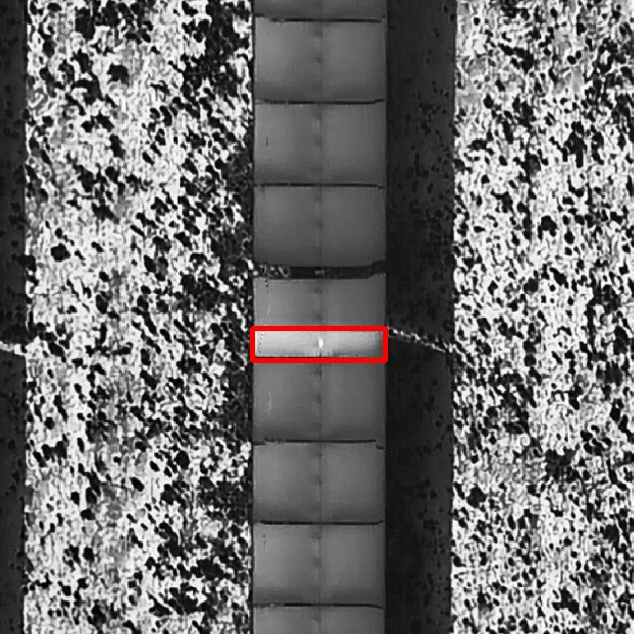
\includegraphics[width=\linewidth]{report_images/faultydiodes_6-68_cropped.jpg}%
\caption{Zoom no defeito: 6-68}%
\end{minipage}%%
\hfill%
\begin{minipage}{0.31\linewidth}%
\centering%
\centering%
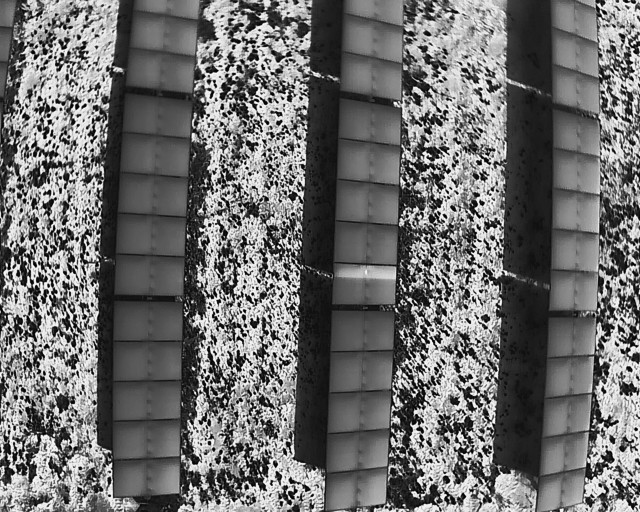
\includegraphics[width=\linewidth]{report_images/faultydiodes_6-68.jpg}%
\caption{Imagem Original: 6-68}%
\end{minipage}%
\end{figure}

%
\FloatBarrier%
No painel 6{-}68 foram detectados diodos de bypass queimados conforme as figuras acima.\newline%
%


\begin{figure}[h!]%
\begin{minipage}{0.31\linewidth}%
\centering%
\centering%
\includegraphics[width=\linewidth]{report_images/faultydiodes_6-26_map.jpg}%
\caption{Localização do defeito: 6-26}%
\end{minipage}%%
\hfill%
\begin{minipage}{0.31\linewidth}%
\centering%
\centering%
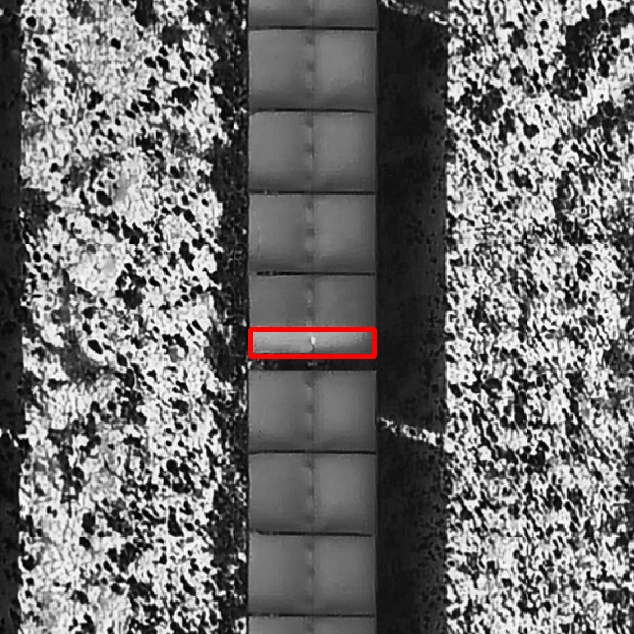
\includegraphics[width=\linewidth]{report_images/faultydiodes_6-26_cropped.jpg}%
\caption{Zoom no defeito: 6-26}%
\end{minipage}%%
\hfill%
\begin{minipage}{0.31\linewidth}%
\centering%
\centering%
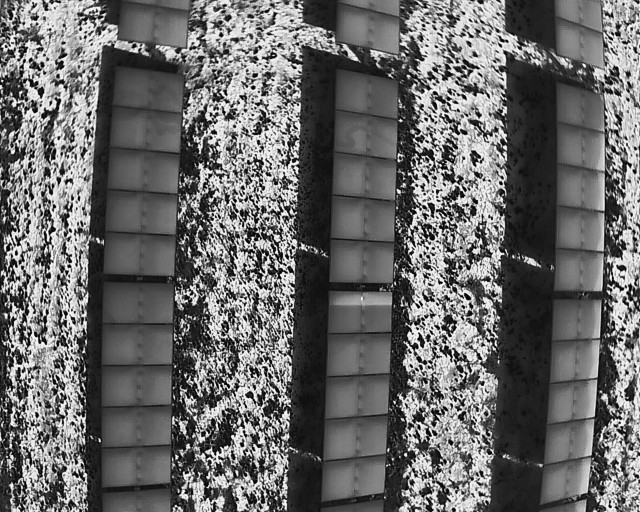
\includegraphics[width=\linewidth]{report_images/faultydiodes_6-26.jpg}%
\caption{Imagem Original: 6-26}%
\end{minipage}%
\end{figure}

%
\FloatBarrier%
No painel 6{-}26 foram detectados diodos de bypass queimados conforme as figuras acima.\newline%
%
\end{document}